\documentclass{article}

\usepackage{amsmath}
\usepackage{amscd}
\usepackage[tableposition=top]{caption}
\usepackage{ifthen}
\usepackage[utf8]{inputenc}
\usepackage{longtable,pdflscape} 
\usepackage{mathptmx}
\usepackage{hyperref}
\usepackage{Sweave}
\usepackage{tikz}
\usepackage{pgf}
\usepackage{a4wide}


% \VignetteIndexEntry{IPMpack: An R Package for demographic modeling}
% \VignetteDepends{Matrix, MASS, nlme, mvtnorm, methods}
% \VignetteKeyword{kwd1}
% \VignetteKeyword{kwd2}

%\SweaveOpts{prefix.string=Guide/} 
 
\begin{document}

\title{IPMpack: an R package for demographic modeling with Integral Projection
Models (v.1.2)}
\author{Jessica Metcalf, Sean M. McMahon, Rob Salguero-Gomez, Eelke Jongejans}
\maketitle


%\section*{IPMpack: an R package for demographic modeling}
%\makeabstract
The goal of IPMpack is to provide a suite of demographic tools based
on Integral Projection Models (IPMs) to support biologists interested in
making projections for populations where demography is strongly linked to a continuous variable, such as size. The package includes functions that can take data, such as size or age, as well as environmental covariates, and build models of growth, survival and fecundity. Functions are defined that then take these
statistical models and construct IPMs. IPMpack has tools that compare different functional forms for the underlying statistical models, plotting them and returning AIC scores, as well as tools for diagnostic tests of the IPM models themselves. There are also methods to build population models for varying environments, use Bayesian methods to sample population parameters,  estimate longevity and passage time, sensitivity and elasticity (of either parameters or matrix elements), and much more.

This vignette is intended to introduce the biologists with a wide range of
quantitative skills to the concepts of IPMs as well as the implementation of
IPMpack.  This vignette is for IPMpack version $2$, and so we encourage users to
contact the IPMpack team at \href{ipmpack@gmail.com}{ipmpack@gmail.com} with
any feedback or mistakes they find.  We also host a blog at R-forge \href{http://ipmpack.r-forge.r-project.org/}{IPMpack Web Site} that contains news of updates, new features, and announcements of papers and meetings relevant to IPMs.
 
\newpage

\section{Introduction to Integral Projection Models}
An Integral Projection Model (IPM) is a demographic tool to explore the dynamics of populations where individuals' fates depend on state variables that are continuous (e.g., weight, diameter at breast height, height, limb length, rosette diameter) or quasi-continuous (e.g., number of leaves, age, number of reproductive structures) and may be a mixture of discrete and continuous. IPMs track the distribution of individuals $n$ across these state variables between census times (e.g., year $t$ and year $t+1$) by projecting from models that define the underlying vital rates (e.g., survival, growth, and reproduction) as a function of the (quasi-)continuous state variables. For detailed introductions to IPMs, see Easterling et al. ($2000$), and Ellner \& Rees ($2006$, $2007$). 

Briefly, an IPM is defined by a kernel $K$ that represents probabilities of growth between discrete or continuous stages, survival across these stages, and the production of offspring and offspring recruitment.   For example, in the simplest case, where the population is structured by a continuous covariate, size, then 
\begin{equation}
n(y, t+1) = \int\limits_{L}^{U} K(y, x) n(x, t) \, dx       
\end{equation}
where $n(y, t+1)$ is the distribution across size $y$ of both established and new individuals in census time $t+1$, $n(x, t)$ the distribution across size of individuals in census time $t$, and $L$ and $U$ the lower and upper size limits modeled in the IPM, respectively. 

 Multiple functional forms for both demographic processes as well as their error structures can be easily accommodated with IPMpack. The $F$ kernel (equation 4) describes per-capita contributions of reproductive individuals to number of new individuals at the next census. Multiple size-dependent or size-independent vital rates can be fitted within the $F$ kernel, reflecting for example reproductive probability, number of reproductive structures (e.g. flowers in plants, basidia in fungi), number of propagules within reproductive structure (e.g. seeds for plants), and so on. Additionally, a range of constants ($c_1$, $c_2$, ...) can be included if there are no data for a stage.  Finally, the $F$ kernel definition includes a probability density function describing the size of offspring recruiting into the population, $f_d$, 
\begin{equation}
n(y, t+1) = \int\limits_{L}^{U} K(y, x) n(x, t) dx = \int\limits_{L}^{U}
[T(y, ) + F(y, x)] n(x, t) dx
\end{equation}

where

\begin{equation}
 \int\limits_{L}^{U} T(y, x) n(x, t) dx = \int\limits_{L}^{U}surv(x)growth(y, x)dx    
\end{equation}

\begin{equation}
 \int\limits_{L}^{U} F(y, x) n(x, t) dx = \int\limits_{L}^{U}
c_1 c_2 c_3 ... fec1(x)fec2(x)fec3(x)...f_d(y, x)dx     
\end{equation}
After numerically solving these kernels, key ecological and evolutionary quantities such as the population rate of increase $\lambda$, the stable population size structure, the net reproductive rate $R_0$, and many others can be estimated (see Caswell $2001$ for more a comprehensive discussion). 

Essentially, the same tools are available for IPMs as for discrete projection matrices (matrix population models), e.g., estimation of population growth rate, sensitivities, elasticities, life table response experiment [LTRE] analyses, passage time calculations, etc (Caswell $2001$, Cochran \& Ellner $1992$, and others). The main difference between an IPM and a matrix model is that while in discrete projection matrices the number of classes (i.e., number of stages in the life cycle of the study species) must be defined {\tt a priori}, IPMs impose the discretization of the three-dimensional surface defined by equation 1 in the last step. This produces a typically large matrix (e.g., $100$ x $100$ cells) that is more robust to biases from matrix dimensionality (Zuidema et al. $2010$, Salguero-Gomez \& Plotkin $2010$) and sample size (Ramula et al. $2009$) than classical matrix models.  

The goal of IPMpack is to provide a centralized set of quantitative techniques
based on IPMs to help ecologists and evolutionary biologists model populations.
IPMpack v. 1.2 can accommodate multiple vital rates from complex life cycles all
grouped into two main sub-kernels: $T$ and $F$ (equation 2) \footnote{Note than in the seminal paper by Easterling et al. ($2000$) this kernel was referred to as $P$, but here we follow the terminology by Caswell ($2001$) and call it $T$ instead). The $T$ kernel (equation 3) describes {\tt growth} between demographic censuses conditional on individuals' survival ({\tt surv}).
}.

This vignette will now walk through the steps of a basic IPM analysis.  We first describe the kind of data necessary to build an IPM.  If a user begins `from scratch', they must input data in a specific format (described below).  However it is possible to jump past this step and use IPMpack capabilities on IPMs that were developed outside of IPMpack.  That is, if a user wants quick diagnostic routines, figures and summary statistics on an IPM matrix already built, IPMpack can readily accommodate that.   However there are some features that, because of the object-oriented coding require some specific structures (and other features that do not).  Please refer to the manual files and the rest of this vignette for this information.  But however a user wants to implement IPMpack, the vignette will begin at the beginning with data set up.  We will then walk through how to build and analyse a basic IPM model.  More complex models will be introduced later, with options to create unique class objects and methods, as well as run comparative model testing and Bayesian implementations.

\section{Getting started: setting up the data for IPMpack}
For users who prefer to define IPM matrices using their own
statistical tools, there is no requirement for the data to be in any
particular format, and most of the functions in IPMpack will operate
on the matrices directly (e.g., life expectancy, sensitivity of matrix
elements, etc).  However, to use IPMpack's full capacities, the
individual-level demographic data must be organized in a specific
format in R: a {\tt data frame} where each row represents one observation of an organism in the population at one census time $t$ with the following column names:  
\begin{itemize}
\item  {\tt size}: size of individuals in census time $t$  $^*$
\item  {\tt sizeNext}: size of individuals in census time $t+1$  $^*$
\item  {\tt surv}: survival of individuals from census time $t$ to  $t+1$ (contains: 0 for death or 1 for survival) $^*$
\item  {\tt fec1, ...}: as many columns as desired relating size to sexual reproduction. For example, this might be: 
  \begin{itemize}
  \item {\tt fec1}: probability of reproduction (output: 0 for no reproductive or 1 for reproductive)
  \item {\tt fec2}: number of reproductive structures (output: 1, 2, 3, $...$) when individual is reproductive, that is, when fec1 = 1
  \item {\tt fec3}: number of propagules (output: 1, 2, 3, $...$) per reproductive structure (e.g. seeds per flower in reproductive plant individual)
  \item ...
  \end{itemize}
  The default construction for the analytical part of IPMpack is such that any columns for which the column label contains $"fec"$ will be included in the analysis of the reproductive part of the life cycle (kernel $F$) automatically. This default can be over-ridden so that specific columns are identified for IPMpack functions to use.   
\item  {\tt stage}: stage of individuals in census time $t$. For rows in the  data frame where {\tt size} is not an NA, then this must be the word ``continuous''. Where {\tt size} is NA, any variety of named discrete stages  may be defined (e.g. ``seed bank''). If this column is missing, many procedures in IPMpack are designed to simply fill in this column assuming that only ``continuous'' state variables describe the life cycle of the species, i.e. there are no discrete stages. 
\item  {\tt stageNext}: stage of individuals in census time $t+1$;  likewise, this column is not essential for many procedures in  IPMpack.  
\item  {\tt number}: number of individuals corresponding to each row in the data frame. For all rows corresponding to movement between continuous stages, this value will be $1$, but for movement between  discrete stages (e.g., from ``dormant seeds'' to ``seeds ready to  germinate'') then this number may be $>1$, potentially directly  reflecting observed individuals in the data. This information avoids having a data frame with a row for every discrete stage (e.g. seed). As above, many  proceedures in IPMpack will simply assume that this value is always 1. 
\item  {\tt covariate}: value of a discrete covariate in census time  $t$, such as light environment at time $t$, age at $t$, patch at $t$, etc. 
\item  {\tt covariateNext}: value of a discrete covariate in census time $t+1$.
\item  ...any other covariates of interest, named as desired by the user are possible too (e.g., precipitation, habitat, temperature, etc).
\end{itemize}

The $^*$ symbol above indicates the minimum columns in the data frame required to obtain passage time and life expectancy calculations. These values form the $T$ kernel. If sufficient additional columns are available, a full life-cycle model, containing the $F$ kernel, can be produced and further analyses are possible.  Although {\tt size} and {\tt sizeNext} can be transformed, many of the utility functions assume no transformations in columns in the original data frame pertaining to fertility. Transformations can be formally called in various parts of the package and appropriate $F$ matrices built that account for these transformations. In addition, users may also define IPMs independently, and then introduce them into IPMpack for application of further utility functions (sensitivities, stochastic growth rates, etc). 


\section{The basics: building an IPM}

First, the user must load the IPMpack package from cran into R. 

\begin{Schunk}
\begin{Sinput}
> #library("IPMpack")
\end{Sinput}
\end{Schunk}
Next, the user must input demographic data. As mentioned above, most functions of IPMpack require a data file with at minimum columns called {\tt size}, {\tt sizeNext}, {\tt surv}, where `size' is size at time t, `sizeNext' is size one census later, and `surv' is a series of 0s and 1s, indicating if the individual survived or not. In the case of `size' and `sizeNext', data can be transformed (e.g., onto a log scale), if appropriate via functions built into IPMpack. For the purpose of learning how to use IPMpack, the user can either use his/her own data (adjusted to have the appropriate headings, as aforementioned), or generate them with a function built into IPMpack:

\begin{Schunk}
\begin{Sinput}
> dff <- generateData()
\end{Sinput}
\end{Schunk}
A quick check indicates that this contains sensible (fictional) information: 
\begin{Schunk}
\begin{Sinput}
> head(dff)
\end{Sinput}
\begin{Soutput}
      size  sizeNext surv covariate covariateNext fec      stage  stageNext
1 8.187547  7.231286    0         1             1   0 continuous continuous
2 4.391269  4.507554    1         1             0   0 continuous continuous
3       NA -1.996332   NA         1             0  NA       <NA> continuous
4 7.141831  6.593043    1         1             0   0 continuous continuous
5       NA -1.910326   NA         1             0  NA       <NA> continuous
6       NA -1.960597   NA         0             0  NA       <NA> continuous
\end{Soutput}
\end{Schunk}

for simplicity, no discrete covariates are included in this first example. Figure~\ref{fig:zero} (p.~\pageref{fig:zero}) is produced by the following code:

\begin{Schunk}
\begin{Sinput}
> plot(dff$size, dff$sizeNext, xlab = "Size at t", ylab = "Size at t+1")
\end{Sinput}
\end{Schunk}
\begin{figure}
\begin{center}
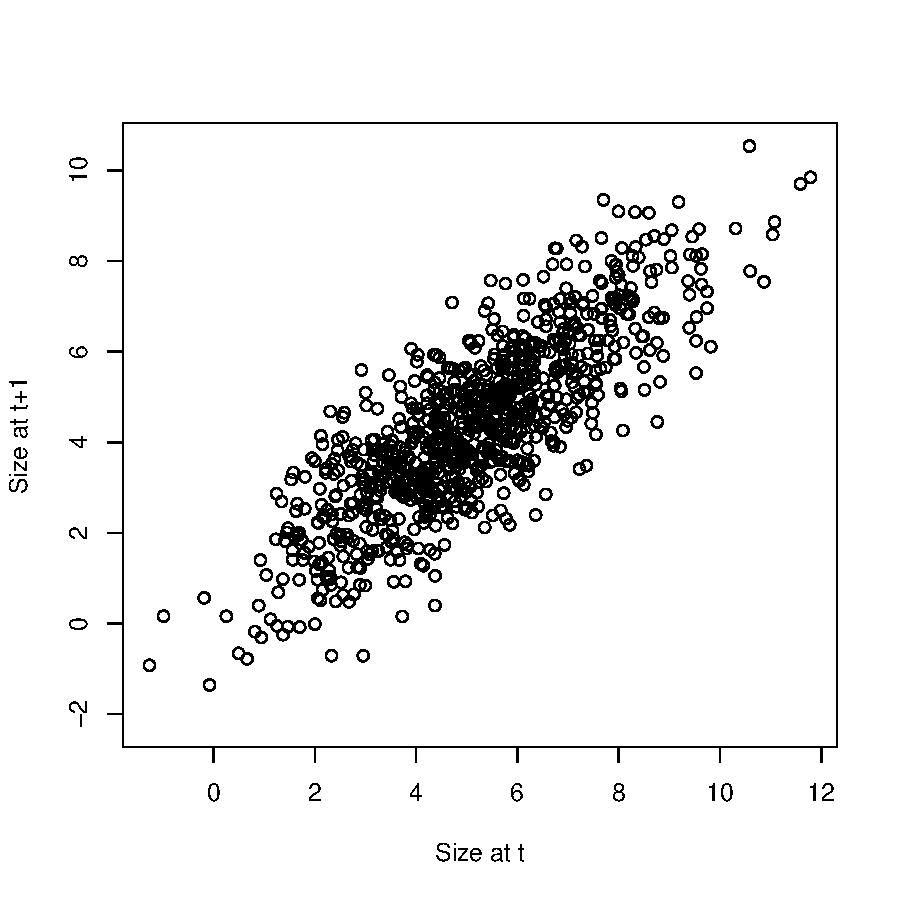
\includegraphics{IPMpack_Vignette-fig0}
\end{center}
\caption{Size at t and size at t+1}
\label{fig:zero}
\end{figure}

IPMpack is written in object-oriented code, using $R$ $S4$ objects. This means that extra object classes are used by IPMpack, with methods assigned to those classes that do particular things to specific objects. An example for those familiar with $R$ is the {\tt plot} function. When applied to two vectors, it produces an x-y plot, but when applied to a fitted linear regression, it provides a series of diagnostic plots. In other words, the 'plot' method is object-specific and does different things to objects of class 'numeric' and objects of class 'lm'. 

IPMpack contains defined classes for growth, survival and fertility objects, and associated methods that allow the user to build IPM objects. In addition, this object-oriented structure in IPMpack uses methods from IPM objects to calculate life expectancy, passage times, and other population estimates of interest. The advantage of object-oriented programming is its flexibility: for example, the same machinery can be applied to suites of underlying regression forms and the user can take advantage of pre-existing highly generalized $R$ functions, such as {\tt predict}. The needs any particular dataset may require different object and method definitions. Towards the end of this vignette we also describe how to define a new class and a new method (e.g., a new growth object for a specific life-history structure, and a new growth method applicable to plotting infomration from that object).

As an example, let us first define objects built as simple polynomial regressions from the generated data. The source code of {\tt generateData} will confirm that the survival data is built around a polynomial logistic regression relating size at $t$ to survival from $t$ to $t+1$, and the growth data is built around a polynomial regression relating size at $t$ to size at $t+1$. To make growth and survival objects that reflect this, the user must implement:  
\begin{Schunk}
\begin{Sinput}
> gr1 <- makeGrowthObj(dataf = dff, explanatoryVariables = "size+size2", 
+ 		   responseType = "sizeNext")
> sv1 <- makeSurvObj(dff, explanatoryVariables = "size+size2")
\end{Sinput}
\end{Schunk}
In both these functions, the argument {\tt explanatoryVariables} contains formulas of the type used in linear or logistic regressions in $R$, built around the possible defined range of transforms of  {\tt size} currently available ({\tt size2} which is size$^2$, {\tt size3} which is size$^3$, and {\tt logsize} which is log(size). Currently further transforms of  {\tt size} are not possible. This function can also be used to fit models that include a single discrete covariate (e.g., light environment, age, etc) as long as this exists in the {\tt dataf} in a column named {\tt covariate}. For instance, the user could model the population dynamics according to  {\tt size + covariate} or  {\tt size + logsize*covariate}, etc. For the growth model, possibilities for {\tt responseType} are: {\tt sizeNext} meaning that the reponse variable is size at the next census time, or {\tt incr} meaning that the response variable is the size increment that has accrued between the two census times (common among tree demographic studies), and {\tt logincr} meaning that the response variable is the log of the size increment that has acrrued between the two census intervals.

Below, the functions {\tt makeGrowthObjManyCov} and {\tt makeSurvObjManyCov} are introduced, which allow any covariates that exist in {\tt dataf} to be fitted (e.g., {\tt size + temperature + site}, etc) via the argument {\tt explanatoryVariables}. The functions are different from the above, since in this case, a slightly different type of growth and survival object needs to be defined to allow slightly different growth and survival methods to be applied. 

Glancing at the source code will confirm that all these functions simply fit a linear regression relating size at t+1 or increment to size at t and covariates for growth, as for survival. The survival and growth objects created have a slot called `fit' that holds the regression.
\begin{Schunk}
\begin{Sinput}
> gr1
\end{Sinput}
\begin{Soutput}
An object of class "growthObj"
Slot "fit":

Call:
lm(formula = Formula, data = dataf)

Coefficients:
(Intercept)         size        size2  
   0.243946     0.817475    -0.002586  
\end{Soutput}
\end{Schunk}
IPMpack contains two functions that allow the user to check these two relationships against the data used for them in order to explore goodness of fit and effect of mesh size, shown in Figure~\ref{fig:one} (p.~\pageref{fig:one}).
\begin{Schunk}
\begin{Sinput}
> par(mfrow = c(1, 2), bty = "l", pty = "m")
> p1 <- picGrow(dff, gr1)
> p2 <- picSurv(dff, sv1, ncuts = 30)
\end{Sinput}
\end{Schunk}
\begin{figure}
\begin{center}
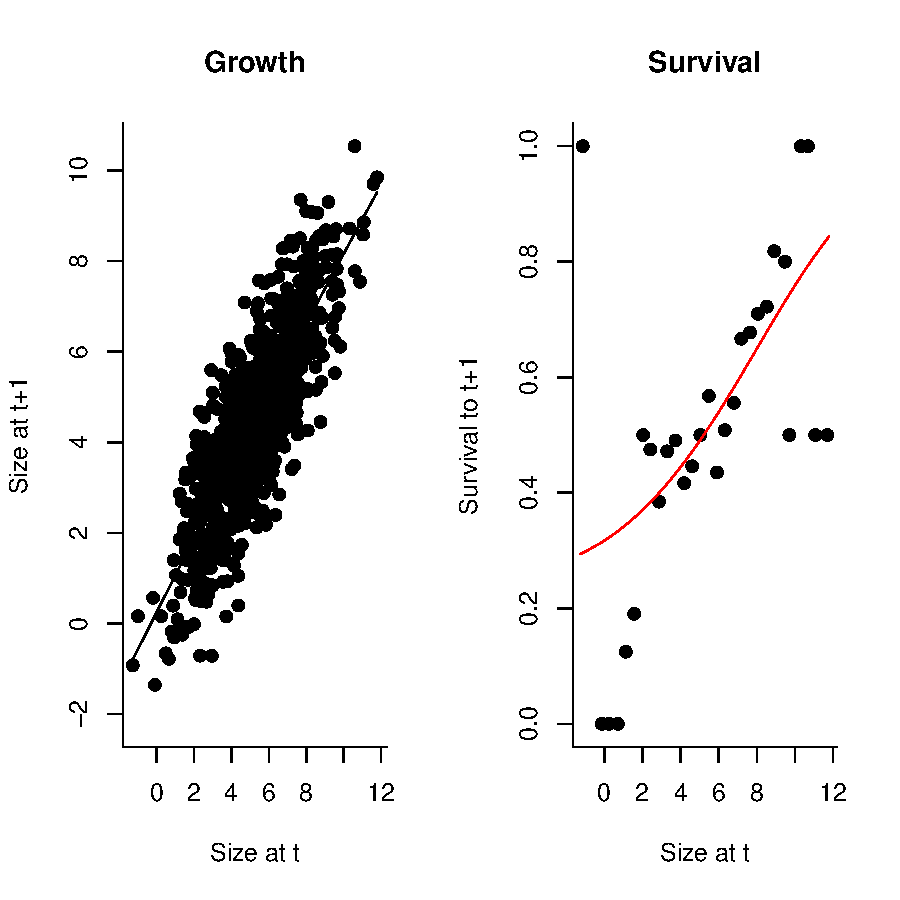
\includegraphics{IPMpack_Vignette-fig1}
\end{center}
\caption{Growth and survival objects}
\label{fig:one}
\end{figure}
To build a demographic model describing survival and growth transitions from these objects, the user can use the function {\tt createIPMPmatrix}, i.e.: 
\begin{Schunk}
\begin{Sinput}
> Pmatrix <- createIPMPmatrix(nBigMatrix = 50, 
+                             minSize = -5, maxSize = 35, 
+                             growObj = gr1, survObj = sv1, 
+                             correction = "constant")
\end{Sinput}
\end{Schunk}
where {\tt nBigMatrix} is the number of bins used, {\tt minSize} and
{\tt maxSize} define the limits of the IPM, $U$ and $L$ in the
equations above. Typically, these range
should usually extend to beyond the smallest and largest size
measurement, but the user might want to exclude outliers). The objects
growObj and survObj define changes in size and survival as defined
above. IPMpack includes an useful function {\tt diagnosticsPmatrix}
that provides a series of plots indicative of whether bin choice and
size range is adequate. Applying this function as a preliminary step
before obtaining demographic and evolutionary output from IPMs is
highly recommended at this stage (see {\tt ?diagnosticsPmatrix} for
details). The argument {\tt correction = "constant"} will rectify some
of the more egregious numerical slippage in the model defined above,
but it will do this in a slightly arbitrary way (i.e. simply adding a
constant value to all elements of each column in the matrix, which may
or may not be appropriate), so it is worth exploring options in detail.

The {\tt createIPMPmatrix} function builds around methods defined so that it will provide appropriate output whatever the survival and growth objects are (e.g. error structure, covariates...). The P matrix contains a matrix defining the transitions, but also other useful slots, e.g., the meshpoints, etc. The user can access this information by writing: 
\begin{Schunk}
\begin{Sinput}
> slotNames(Pmatrix)
\end{Sinput}
\begin{Soutput}
[1] ".Data"          "nDiscrete"      "nEnvClass"      "nBigMatrix"    
[5] "meshpoints"     "env.index"      "names.discrete"
\end{Soutput}
\end{Schunk}
and finally, the user can plot the Pmatrix using {\tt persp} (Figure~\ref{fig:two}). 
\begin{figure}
\begin{center}
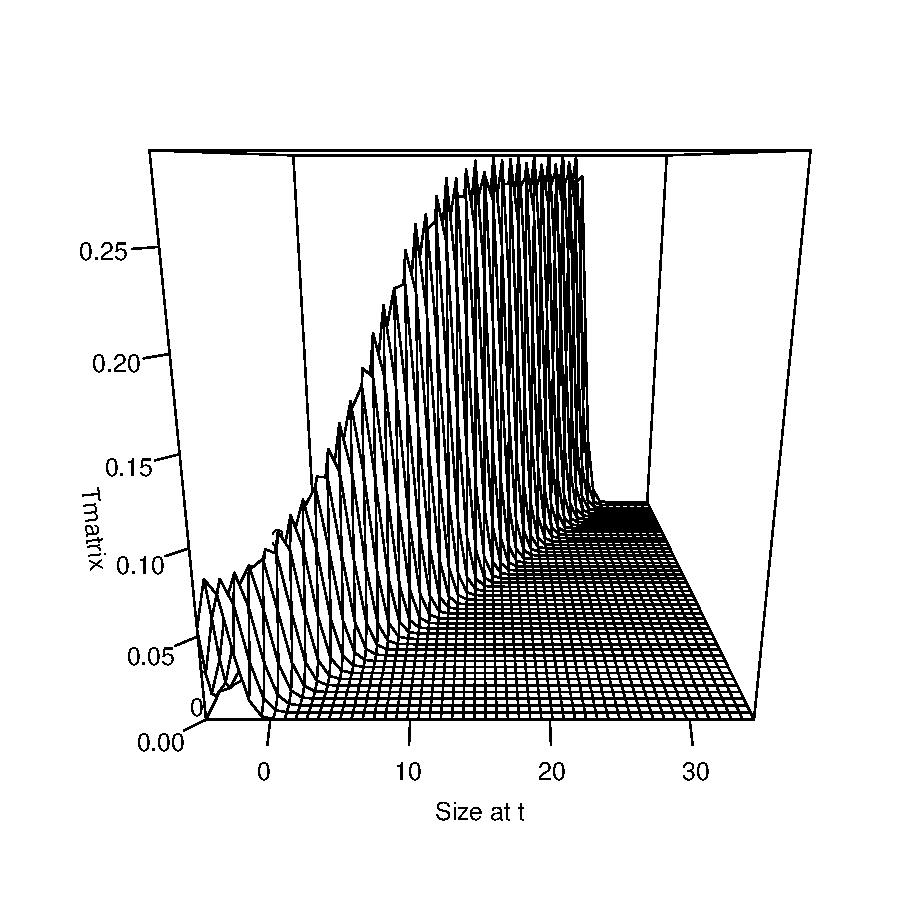
\includegraphics{IPMpack_Vignette-fig2}
\end{center}
\caption{Transition matrix encompassing survival and growth transitions only}
\label{fig:two}
\end{figure}
Next, with this, the user can obtain the life expectancy, and passage time to a chosen size (here set at the mean) for the range of meshpoints
\begin{Schunk}
\begin{Sinput}
> LE <- meanLifeExpect(Pmatrix)
> pTime <- passageTime(mean(dff$size, na.rm = TRUE), Pmatrix)
\end{Sinput}
\end{Schunk}
and the user can also plot these againts {\tt Pmatrix@meshpoints} to examine how life expectancy and passage vary as a function of size (Figure~\ref{fig:three} p.~\pageref{fig:three}).
\begin{figure}
\begin{center}
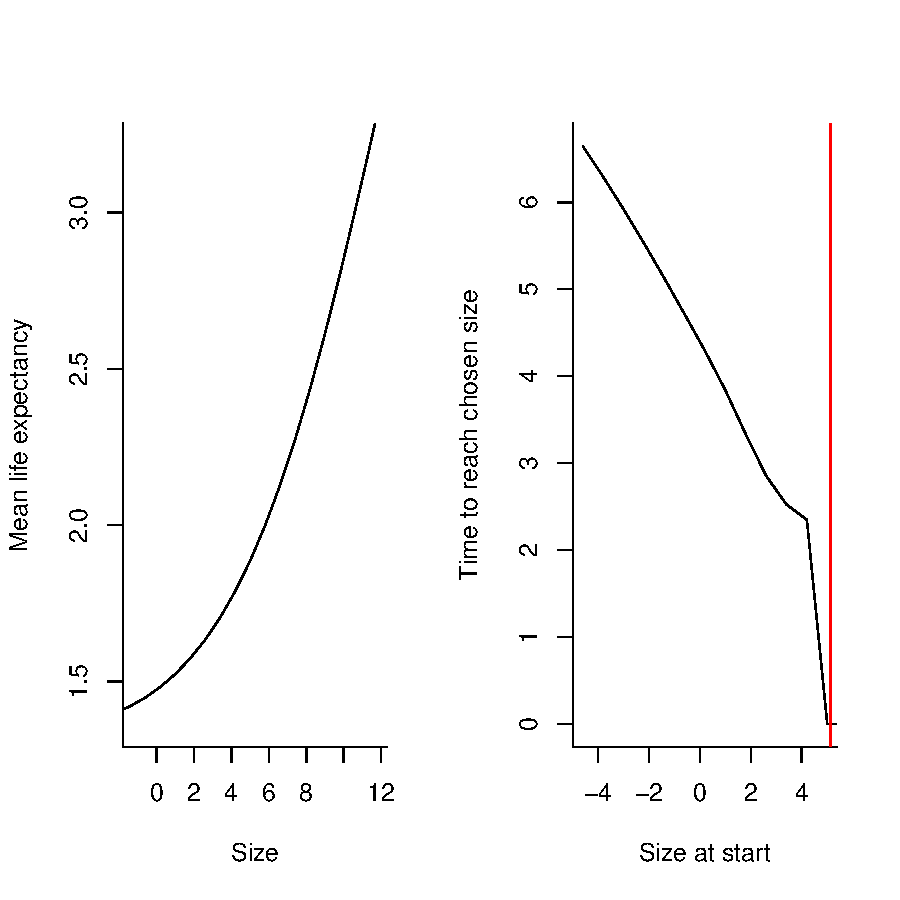
\includegraphics{IPMpack_Vignette-fig3}
\end{center}
\caption{Associated Life Expectancy and Passage Time}
\label{fig:three}
\end{figure}
The function {\tt run.Simple.Model} takes as minimum arguments a data frame and a target size (i.e., here type: {\tt runSimpleModel(dff, chosenSize = 4)}) and runs this analysis to create figures for survival, growth, life expectancy and passage time as shown so far, assuming the simplest possible models of survival and growth (basic linear and logistic regressions, no covariates, etc).

If the user defines a fertility object -which for instance is not always easy with for example trees- IPMpack can also create a transition matrix describing movement between sizes attributable to fertility.
\begin{Schunk}
\begin{Sinput}
> fv1 <- makeFecObj(dff, explanatoryVariables = "size", 	
+                   Family = "gaussian", 
+                   Transform = "log")
> Fmatrix <- createIPMFmatrix(nBigMatrix = 50, minSize = -5,
+                             maxSize = 35, 
+                             fecObj = fv1, 
+                             correction = "constant")
\end{Sinput}
\end{Schunk}
Note that {\tt makeFecObj} can either just scan the {\tt dataf} and extract all the columns that contain the letters "fec" (the default, as explained above) and fit them in alphabetical sequence using the predictors defined in {\tt explanatoryVariables} and using the family defined in {\tt Family} with transforms defined in {\tt Transform} (in the alphabetical sequence); or {\tt fecNames} can be defined in an argument to {\tt makeFecObj}, and this tells $R$ which columns to select and fit fertility predictors to as in the previous, where {\tt Family}, {\tt Transform} etc, will be applied in the order {\tt fecNames}. Please note that the fecundity columns must not be transformed in the data frame if {\tt makeFecObj} function is used since IPMpack will perform appropriate transformations in the fitting according to the argument {\tt Transform} and will use these appropriately in functions designed to build the F matrix. 

The user can combine the F matrix with (an identically built, i.e., same bin number, size limits and discrete classes) survival-growth transition P matrix to
obtain a full Integral Projection Model, and its population growth rate $\lambda$, sensitivity, elasticity, etc. 
\begin{Schunk}
\begin{Sinput}
> IPM <- Pmatrix + Fmatrix
> eigen(IPM)$value[1]
\end{Sinput}
\begin{Soutput}
[1] 0.7841919
\end{Soutput}
\begin{Sinput}
> sensitivity <- sens(IPM)
> elasticity <- elas(IPM)
\end{Sinput}
\end{Schunk}
These outputs can be plotted against the meshpoints (Figure~\ref{fig:four} p.~\pageref{fig:four}).
\begin{figure}
\begin{center}
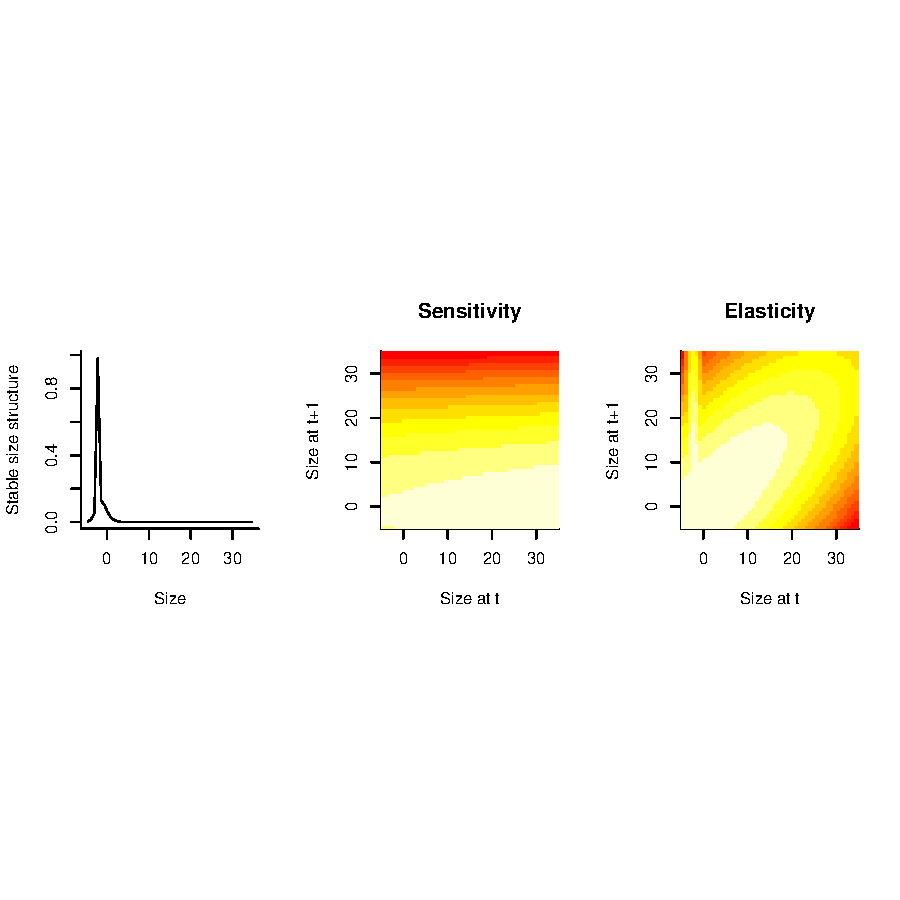
\includegraphics{IPMpack_Vignette-fig4}
\end{center}
\caption{Measures off a full IPM}
\label{fig:four}
\end{figure}
In addition to perturbation measures from mesh cells, the user can also obtain sensitivity and elasticity of particular parameters that underlie the kernels, e.g., doing:
\begin{Schunk}
\begin{Sinput}
> res <- sensParams(growObj = gr1, survObj = sv1, fecObj = fv1, 
+                   nBigMatrix = 50, minSize = -5, maxSize = 15)
> res
\end{Sinput}
\begin{Soutput}
$slam
    grow (Intercept)            grow size           grow size2 
           0.1312423           -0.2037815            0.4537052 
           sd growth     surv (Intercept)            surv size 
         -20.1796339            0.2657089           -0.4217758 
          surv size2 reprod 1 (Intercept)        reprod 1 size 
           0.9221942            0.7313364           -1.2206462 

$elam
    grow (Intercept)            grow size           grow size2 
         0.032017661         -0.166594709         -0.001173462 
           sd growth     surv (Intercept)            surv size 
       -22.001080487         -0.203850453         -0.041742495 
          surv size2 reprod 1 (Intercept)        reprod 1 size 
         0.008527461         -0.093363768         -0.426715381 
\end{Soutput}
\begin{Sinput}
> plot(1:10)
\end{Sinput}
\end{Schunk}
and this output can be plotted out (Figure~\ref{fig:foura} p.~\pageref{fig:foura}) using
\begin{Schunk}
\begin{Sinput}
> par(mfrow = c(2, 1), bty = "l", pty = "m")
> barplot(res$slam, main = expression("Parameter sensitivity of "*lambda), 
+ 		    las = 2, cex.names = 0.5)
> barplot(res$elam, main = expression("Parameter elasticity of "*lambda), 
+ 		    las = 2, cex.names = 0.5)
> plot(1:10)
\end{Sinput}
\end{Schunk}
\begin{figure}
\begin{center}
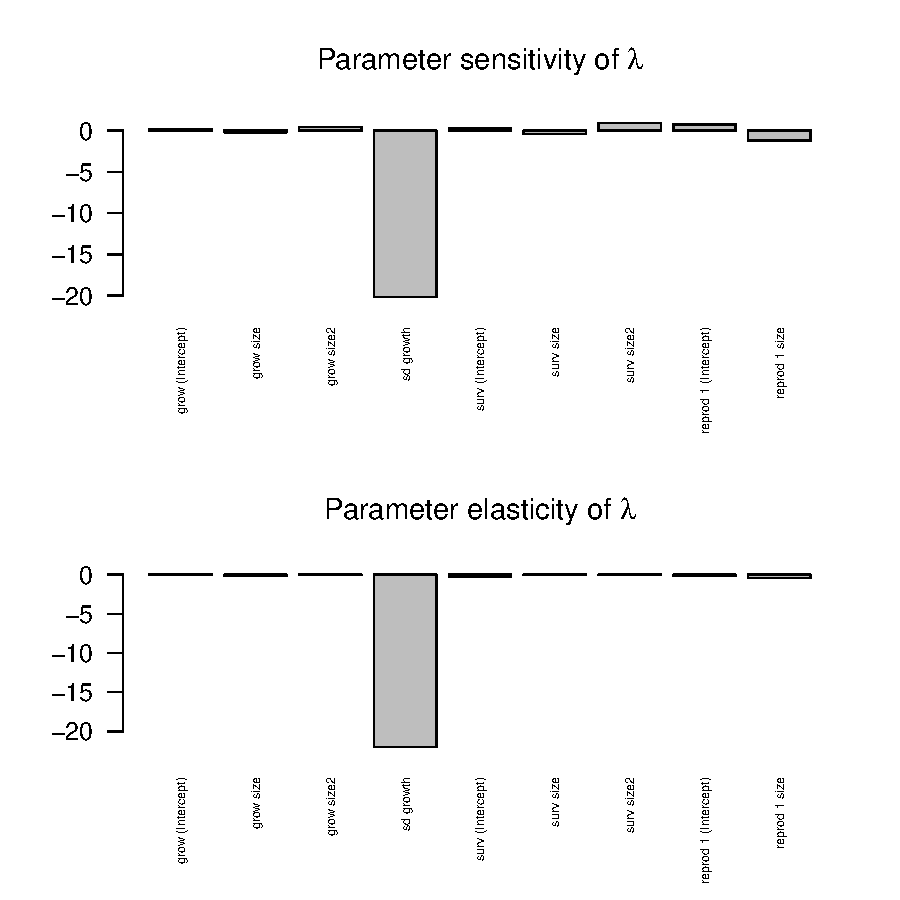
\includegraphics{IPMpack_Vignette-fig4a}
\end{center}
\caption{Sensitivity and elasticity of parameter values}
\label{fig:foura}
\end{figure}
%Similar code could be developed to explore sensitivity of other emergent %measures, e.g., mean passage time, etc. 

\section{Discretely varying environments}
A first possible extension of IPMs is to create a compound IPM matrix where, in addition to moving between continuous sizes, individuals move through discrete environments where the discrete environmental states have an expected sequence, and therefore can be described by a transition matrix of their own (e.g. light environments for tropical trees, as in Metcalf et al. $2009$). 

To explore this type of dynamics, the user needs to either provide or simulate an environmental variable at $t$ and the corresponding value at $t+1$. Here, it has been generated as part of the {\tt generateData} function (See above). From this generated data, the user can then create an environmental transition matrix, which describes how the environment tends to move between these states from one census time to the next. If the data has been set up as described, there is a function that will do this for the user: 
\begin{Schunk}
\begin{Sinput}
> env1 <- makeEnvObj(dff) 
> env1
\end{Sinput}
\begin{Soutput}
An object of class "envMatrix"
          [,1]      [,2]
[1,] 0.2168525 0.2020725
[2,] 0.7831475 0.7979275
Slot "nEnvClass":
[1] 2
\end{Soutput}
\end{Schunk}
The user can now use IPMpack to create a survival-growth transition P matrix that encompasses movement across environments, first redefining the survival and growth
objects to fit a discrete covariate, by changing the {\tt explanatoryVariables} argument: 
\begin{Schunk}
\begin{Sinput}
> gr1 <- makeGrowthObj(dff, explanatoryVariables = "size+covariate")
> sv1 <- makeSurvObj(dff, explanatoryVariables = "size+covariate")
\end{Sinput}
\end{Schunk}
Note that these functions will only work appropriately for a discrete covariate if the value of the covariate at time $t$ is available as a column in the data frame names {\tt covariate} and the value of the covariate at the next census is available as a column in the data frame called {\tt covariateNext}. IPMpack functions use the presence of a column in the data frame called {\tt covariate} as a cue to renumber values in these two columns to numeric levels between 1 and the observed number of covariate levels to facilitate looping, and changes them into factors. Once this step is implemented, the user can use these functions to create a compound P matrix, using {\tt createCompoundPmatrix}: 
\begin{Schunk}
\begin{Sinput}
> Pmatrix <- createCompoundPmatrix(nBigMatrix = 50, minSize = -5, 
+                                  maxSize = 35, 
+                                  envMatrix = env1, growObj = gr1, 
+                                  survObj = sv1, 
+                                  correction = "constant")
\end{Sinput}
\end{Schunk}
Essentially, the compound P matrix is a large matrix with stacked IPMs
corresponding to each environment, modified to reflect movement
between environmental states defined by {\ env1}. Passage time can be
calculated using similar function, but now including the environmental
matrix as an argument (equivalent life expectancy functions are in development): 
\begin{Schunk}
\begin{Sinput}
> pTimes <- stochPassageTime(Pmatrix@meshpoints[15], Pmatrix, env1)
\end{Sinput}
\end{Schunk}
The resulting vectors contain the life expectancy and time to reach each size for individuals starting in each different environmental class, concatenated together (i.e. there are {\tt nBigMatrix} values in the LE matrix ranging over the first environment, then {\tt nBigMatrix} values ranging over the second environment, etc). The user can plot these against meshpoints 
(Figure~\ref{fig:five} p.~\pageref{fig:five}), 
each colour indicates a different starting environment. Similar syntax can be used for passage time (although note that here the function name has changed).  

(Figure~\ref{fig:five}) : 
\begin{figure}
\begin{center}
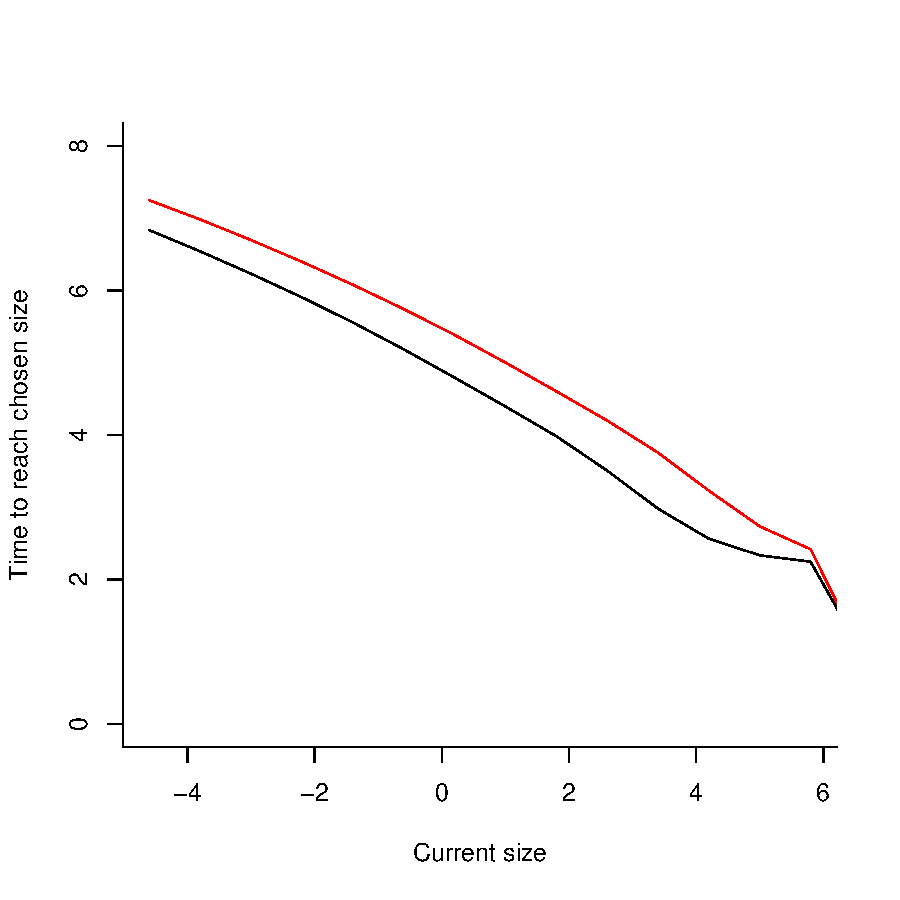
\includegraphics{IPMpack_Vignette-fig5}
\end{center}
\caption{Life expectancy and passage time for a compound IPM;   different colours reflect predictions for individuals starting in different environments}
\label{fig:five}
\end{figure}

With a fertility object, the user can also define a full life cycle IPM model for this environment. With such an information, obtaining the stochastic population rate of increase $\lambda_s$ in this environment is relatively straight-forward. IPMpack does this by sampling a very large number of environments and corresponding IPMs, and multiplying them together (Childs et al. $2004$). At the moment, this is only defined for the case where environments (defined by the discrete covariates) are distributed independently (i.e. the next state does not depend on the previous state). To do this, the user must first define a list of IPMs (each the sum of a matrix of survival-growth transitions, and a matrix of fecundity transitions corresponding to a particular environment): 
\begin{Schunk}
\begin{Sinput}
> IPMlist <- makeListIPMs(dataf = dff, nBigMatrix = 25, minSize = -5, 
+                         maxSize = 35, explSurv = "size+covariate", 
+                         explGrow = "size+size2+covariate", 
+                         explFec = "size", Transform="log",correction = "constant")
\end{Sinput}
\end{Schunk}
Note that in this example IPMpack uses an arbitrary selection of
explanatory variables for all the various linear and logistic
regressions ({\tt explGrow}, {\tt explSurv}, etc). In reality, careful
model selection will be used to establish this. Additionally, the
number of environment types should in principle be greater than the
two or three used here. Next, the user can estimate $\lambda_s$ using: 
\begin{Schunk}
\begin{Sinput}
> stochGrowthRateSampleList(listIPMmatrix = IPMlist, 
+                           nRunIn = 30, tMax = 50)
\end{Sinput}
\begin{Soutput}
[1] -0.4577622
\end{Soutput}
\end{Schunk}
where {\tt nRunIn} defines the number of time steps to discard from the start of the time series in order to remove transient dynamics, and {\tt tMax} is the total
number of time steps to run, and should be large enough that increasing it does not substantially change the result (numbers presented here for efficiency are almost certaintly not large enough). 

%Simply taking the eigenvalue of the sum to the compound $T$ and $F$ matrices will
%provide a sligthly different result given Jensen's inequality. %%check
                                %%this... read Tulja + Carol stoch
                                %%elastivity paper. 

\section{More generally varying environments}

An alternative way of inhabiting stochastic environments is to experience continuously changing covariates (rather than moving between discrete states, as the above describes). In this case, rather than building a single megamatrix, desired variables are obtained by multiplying up a suite of matrices and relying on the weak
ergodic theorem for convergence (as described for obtaining $\lambda_s$, above). IPMpack contains code to do this. The user must first define a new data frame containing several time-varying covariates, and then, build the associated survival, growth and fertility objects: 
\begin{Schunk}
\begin{Sinput}
> dff <- generateDataStoch()
> sv1 <- makeSurvObjManyCov(dataf = dff, 
+                           explanatoryVariables = "size+covariate1+covariate3")
> gr1 <- makeGrowthObjManyCov(dataf = dff, 
+                             explanatoryVariables = "size+covariate1+covariate2")
> fv1 <- makeFecObj(dataf = dff, fecConstants = data.frame(1.8), 
+                   explanatoryVariables = "size", Transform = "log")
\end{Sinput}
\end{Schunk}
As before, the user can explore the data: 
\begin{Schunk}
\begin{Sinput}
> head(dff)
\end{Sinput}
\begin{Soutput}
      size  sizeNext surv covariate1 covariate2 covariate3       fec      stage
1 5.317636  9.193815    0  1.1032548 -0.5851448  1.0414388 20.336722 continuous
2 3.297403  7.825271    0  1.3045531  1.3406407  0.2128416  0.000000 continuous
3 5.058010  4.057263    1 -0.5289626  0.4839539  0.2280878 11.402339 continuous
4 6.615050 11.158390    0  1.4043558 -0.2104289 -0.6447409  6.534707 continuous
5 7.794640  5.728984    0 -0.9192372 -0.7479364  1.1978393 14.624768 continuous
6 6.571999  5.317525    1 -0.5234180  2.0311775  0.7783156 11.915277 continuous
   stageNext number
1 continuous      1
2 continuous      1
3 continuous      1
4 continuous      1
5 continuous      1
6 continuous      1
\end{Soutput}
\end{Schunk}
and glance at the objects, e.g., 
\begin{Schunk}
\begin{Sinput}
> gr1
\end{Sinput}
\begin{Soutput}
An object of class "growthObjMultiCov"
Slot "fit":

Call:
lm(formula = Formula, data = dataf)

Coefficients:
(Intercept)         size   covariate1   covariate2  
    1.02213      0.89829      2.98623      0.01061  
\end{Soutput}
\end{Schunk}
From these data, to explore predicted demographic outcomes for the model, the user must decide on a time scale and length for investigation, and define it by a vector called `tVals', here set to reflect monthly intervals over $4$ years, with years as the time scale. With this, the user can then generate a time series that should look like the time series observed in the data. In the example below, covariates that vary seasonally were simulated, i.e., they fluctuates randomly around a sine wave which peaks once a year (`covTest'), and from this generate a matrix containing time as rows, and different covariates in columns.  
\begin{Schunk}
\begin{Sinput}
> tVals <- seq(1, 4, by = 1/12)
> covTest <- c(1 + 0.5*sin(2*pi*tVals))
> covMatTest <- data.frame(covariate1 = rnorm(length(covTest), covTest, 0.5) - 1, 
+                          covariate2 = rnorm(length(covTest), covTest, 0.5) - 1, 
+                          covariate3 = rnorm(length(covTest), covTest, 0.5) - 1)
\end{Sinput}
\end{Schunk}
Note that  if there is no apparent temporal pattern to the data one could simply generate random normal distributions of the covariates using their observed
mean and variance. Other types of temporal patterns (multiannual, etc) are also possible. With this setup, the user can then estimate the stochastic growth rate over these years, using the geometric mean of the population growth rate (Tuljapurkar $1990$; Childs et al. $2004$), for these particular covariates using:
\begin{Schunk}
\begin{Sinput}
> r <- stochGrowthRateManyCov(covariate = covMatTest, nRunIn = 12*1, 
+                             tMax = length(tVals), growthObj = gr1, 
+                             survObj = sv1, fecObj = fv1, nBigMatrix = 20, 
+                             minSize = 2*min(dff$size, na.rm = TRUE), 
+                             maxSize = 1.5*max(dff$size, na.rm = TRUE), 
+                             nMicrosites = 50, correction = "constant")
> print(r)
\end{Sinput}
\begin{Soutput}
[1] 0.4808031
\end{Soutput}
\end{Schunk}
Setting nRunIn = $12*1$ in this example is equivalent to discarding the first $1$ years (likely to contain transients) since the chosen time step is months. Note that in this formula, it was assumed that density-dependence acts on seedling establishment, and that $50$ microsites are available for seedling establishment in every time step. Setting nMicrosites = $0$ allows for calculations without density-dependence, and nMicrosites can also be a vector, if the number of microsites fluctuates through time. It may also be interesting to have a glance at what has been happening to the population structure over this time-course, and the function {\tt trackPopStructManyCov} allows this; IPMpack also contains a dedicated function to depict the results from this, {\tt plotResultsStochStruct}.

\section{Incorporating discrete stages}
Populations are often structured by both discrete and a continuous stages, for example, many plant populations may persist for many years in a seedbank as well as having size-determined fates after they germinate. IPMpack can incorporate this variability for complex life cycles (Ellner \& Rees $2006$). To illustrate this, the user must first generate data that includes both discrete and continuous life-history stages:
\begin{Schunk}
\begin{Sinput}
> dff <- generateDataDiscrete()
\end{Sinput}
\end{Schunk}
A quick check indicates that these data contain several types of stage classification (and not just "continuous" as seen up till now):
\begin{Schunk}
\begin{Sinput}
> table(dff$stage)
\end{Sinput}
\begin{Soutput}
continuous    dormant   seedAge1    seedOld 
       950         50         35         32 
\end{Soutput}
\end{Schunk}
Given this data structure, the user can make a fertiliy object that reflects the fact that propagules (e.g., seeds) produced in one year may directly recruit into the continuous phase (e.g., seedling), or may end up in a discrete stage (e.g., seed bank). The {\tt makeFecObj} (and similar functions) have an argument that allows the user to define this dichotomy, called {\tt offspringSplitter}:
\begin{Schunk}
\begin{Sinput}
> fv1 <- makeFecObj(dataf = dff, Transform = "log", 
+                   offspringSplitter = data.frame(continuous = 0.2, 
+                   dormant = 0, seedAge1 = 0.8, seedOld = 0), 
+                   fecByDiscrete = data.frame(dormant = 0, 
+                   seedAge1 = 0, seedOld = 0))
\end{Sinput}
\end{Schunk}
In this example, 20 \% of seeds produced at $t$ end up in the continuous part of the population structure at $t+1$ (for example, they might directly recruit as rosettes from one year to the next) and 80 \% of seeds recruit into the "one year old seeds" stage. Although in this case no individuals are recruited at $t+1$ into the "dormant" or "old seeds" stages (since these will come from adult plants or the seed bank), they are included as {\tt offspringSplitter} is where IPMpack identifies all the existing discrete stages. The argument {\tt fecByDiscrete} reflects the fact that none of the discrete classes addressed in this example are likely to directly produce offspring (which may not always be the case). The resulting fecundity object can be used with {\tt createIPMFmatrix} in the usual way:
\begin{Schunk}
\begin{Sinput}
> Fmatrix <- createIPMFmatrix(fecObj = fv1, nBigMatrix = 5, 
+                             minSize = min(dff$size, na.rm = TRUE), 
+                             maxSize = max(dff$size, na.rm = TRUE), 
+                             correction = "constant")
\end{Sinput}
\end{Schunk}
The user also needs a {\tt Pmatrix} that reflects the same structure. The continuous part of the P matrix will be broadly the same as usual:
\begin{Schunk}
\begin{Sinput}
> gr1 <- makeGrowthObj(dataf = dff, 
+                      explanatoryVariables = "size", responseType = "sizeNext")
> sv1 <- makeSurvObj(dff, explanatoryVariables = "size")
\end{Sinput}
\end{Schunk}
Movement in and out of discrete stages is defined via an add-on of a transition matrix, that is defined using: 
\begin{Schunk}
\begin{Sinput}
> discTrans <- makeDiscreteTrans(dff)
\end{Sinput}
\end{Schunk}
which captures survival and transitions between discrete stages and the continuous stage (note that this function will not work unless the data frame {\tt dff} contains appropriate columns {\tt stage} and {\tt stageNext}) and then the user can construct the P matrix using: 
\begin{Schunk}
\begin{Sinput}
> Pmatrix <- createIPMPmatrix(nBigMatrix = 5, 	
+                             growObj = makeGrowthObj(dff), 
+                             survObj = makeSurvObj(dff), 
+                             discreteTrans = discTrans, 
+                             correction = "constant")
\end{Sinput}
\end{Schunk}
Note that both the P matrix and the F matrix in this example have a rather small number of bins just for ease of comparison, and that a higher number is almost certainly advisable. The user can examine both matrices: 
\begin{Schunk}
\begin{Sinput}
> print(Pmatrix)
\end{Sinput}
\begin{Soutput}
An object of class "IPMmatrix"
              [,1]         [,2]          [,3]          [,4]          [,5]
[1,]  3.000000e-01 0.000000e+00  0.000000e+00  1.061834e-02  3.083104e-01
[2,]  0.000000e+00 0.000000e+00  0.000000e+00  0.000000e+00  0.000000e+00
[3,]  0.000000e+00 4.439560e-01  4.323308e-01  0.000000e+00  0.000000e+00
[4,]  6.999642e-01 7.252741e-02  1.127820e-01  4.629766e-01  2.186584e-16
[5,]  3.579026e-05 6.218594e-08  1.610992e-09  6.298853e-22  2.569937e-03
[6,]  8.654581e-27 4.186000e-24  1.825427e-29  5.683256e-87  2.003144e-34
[7,]  9.897362e-66 2.212194e-50  1.640789e-61 3.400684e-196 1.035464e-109
[8,] 5.352850e-122 9.178342e-87 1.169926e-105  0.000000e+00 3.549698e-229
              [,6]          [,7]          [,8]
[1,]  1.174315e-03  1.592486e-08  2.220446e-16
[2,]  0.000000e+00  0.000000e+00  0.000000e+00
[3,]  0.000000e+00  0.000000e+00  0.000000e+00
[4,]  5.547463e-62 6.930333e-142 3.885314e-244
[5,]  5.632545e-15  6.078806e-61 2.944044e-129
[6,]  3.792698e-12  3.536029e-24  1.479434e-58
[7,]  1.693656e-53  1.364101e-31  4.930381e-32
[8,] 5.015744e-139  3.489882e-83  1.089679e-49
Slot "nDiscrete":
[1] 3

Slot "nEnvClass":
[1] 1

Slot "nBigMatrix":
[1] 5

Slot "meshpoints":
[1]  4.1 14.3 24.5 34.7 44.9

Slot "env.index":
[1] 1 1 1 1 1

Slot "names.discrete":
[1] "dormant"  "seedAge1" "seedOld" 
\end{Soutput}
\begin{Sinput}
> print(Fmatrix)
\end{Sinput}
\begin{Soutput}
An object of class "IPMmatrix"
     [,1] [,2] [,3]         [,4]         [,5]         [,6]         [,7]
[1,]    0    0    0 0.000000e+00 0.0000000000 0.0000000000 0.0000000000
[2,]    0    0    0 7.767925e-02 0.1638155587 0.3454659872 0.7285434260
[3,]    0    0    0 0.000000e+00 0.0000000000 0.0000000000 0.0000000000
[4,]    0    0    0 1.556169e-03 0.0032817597 0.0069208101 0.0145951001
[5,]    0    0    0 7.865908e-03 0.0165881905 0.0349823647 0.0737733172
[6,]    0    0    0 8.174445e-03 0.0172388563 0.0363545353 0.0766670487
[7,]    0    0    0 1.746566e-03 0.0036832830 0.0077675710 0.0163808102
[8,]    0    0    0 7.672356e-05 0.0001618001 0.0003412157 0.0007195802
            [,8]
[1,] 0.000000000
[2,] 1.536404576
[3,] 0.000000000
[4,] 0.030779193
[5,] 0.155578457
[6,] 0.161680965
[7,] 0.034545026
[8,] 0.001517502
Slot "nDiscrete":
[1] 3

Slot "nEnvClass":
[1] 1

Slot "nBigMatrix":
[1] 5

Slot "meshpoints":
[1] -0.9043241  1.6920777  4.2884795  6.8848813  9.4812831

Slot "env.index":
[1] 1 1 1 1 1

Slot "names.discrete":
[1] "dormant"  "seedAge1" "seedOld" 
\end{Soutput}
\end{Schunk}
and check for example that the slot {\tt namesDiscrete} is aligned between them, and add them together: 
\begin{Schunk}
\begin{Sinput}
> print(Pmatrix+Fmatrix)
\end{Sinput}
\begin{Soutput}
              [,1]         [,2]          [,3]         [,4]         [,5]
[1,]  3.000000e-01 0.000000e+00  0.000000e+00 1.061834e-02 0.3083103589
[2,]  0.000000e+00 0.000000e+00  0.000000e+00 7.767925e-02 0.1638155587
[3,]  0.000000e+00 4.439560e-01  4.323308e-01 0.000000e+00 0.0000000000
[4,]  6.999642e-01 7.252741e-02  1.127820e-01 4.645328e-01 0.0032817597
[5,]  3.579026e-05 6.218594e-08  1.610992e-09 7.865908e-03 0.0191581277
[6,]  8.654581e-27 4.186000e-24  1.825427e-29 8.174445e-03 0.0172388563
[7,]  9.897362e-66 2.212194e-50  1.640789e-61 1.746566e-03 0.0036832830
[8,] 5.352850e-122 9.178342e-87 1.169926e-105 7.672356e-05 0.0001618001
             [,6]         [,7]         [,8]
[1,] 0.0011743145 1.592486e-08 2.220446e-16
[2,] 0.3454659872 7.285434e-01 1.536405e+00
[3,] 0.0000000000 0.000000e+00 0.000000e+00
[4,] 0.0069208101 1.459510e-02 3.077919e-02
[5,] 0.0349823647 7.377332e-02 1.555785e-01
[6,] 0.0363545353 7.666705e-02 1.616810e-01
[7,] 0.0077675710 1.638081e-02 3.454503e-02
[8,] 0.0003412157 7.195802e-04 1.517502e-03
\end{Soutput}
\end{Schunk}
The first three rows and columns concern transitions in and out of the discrete stages; the remainder are the usual T and F matrices describing moving across the continuous variables. The usual types of calculations (sensitivity via {\tt sens}, life expectancy via {\tt meanLifeExpect}, etc) can be applied here too.    


\section{Parameter uncertainty in a constant environment}

First, the user must generate data again, and from them, a list of survival and growth objects reflecting the parameter posteriors of the fitted linear and logistic regression (taking the simplest case of structure only via a continuous covariate):
\begin{Schunk}
\begin{Sinput}
> dff <- generateData()
> grlist <- makePostGrowthObjs(dff, 
+                              explanatoryVariables = "size", 
+                              burnin=20,nitt = 40)
> svlist <- makePostSurvivalObjs(dff, 
+                                explanatoryVariables = "size", 
+                                burnin=20,nitt = 40)
\end{Sinput}
\end{Schunk}
Note that the data must not contain NAs. This function can also be used to set priors, etc. Note that the number of samples from the posterior used here {\tt nitt} is rather small, and larger numbers are advisable. With output from this, the user can make lists of the P matrices:
\begin{Schunk}
\begin{Sinput}
> PmatrixList <- makeListPmatrix(grlist, svlist, nBigMatrix = 20, 
+                                minSize = -5, 
+                                maxSize = 35, 
+                                correction = "constant")
\end{Sinput}
\end{Schunk}
If one of the lists is longer than the other, this function samples the shorter object at random to reach the size of the longer object. Note that in this example the matrix size is rather small just to save time, and larger number of bins are advisable. The function will also construct compound matrices, if an environmental
matrix is provided. With this, the user can now obtain some posteriors for constant environment models. 
\begin{Schunk}
\begin{Sinput}
> res <- getIPMoutput(PmatrixList, targetSize = 5, FmatrixList = NULL)
> names(res)
\end{Sinput}
\begin{Soutput}
[1] "LE"          "pTime"       "lambda"      "stableStage"
\end{Soutput}
\end{Schunk}
The vector called $\lambda$ and matrix called stableSize, etc, will consist of NAs, unless a list of Fmatrices is also provided, so that a complete population projection matrix can be built. IPMpack contains a similar function to obtain a list of F matrices, and if such a list is included as the third argument into the function {\tt getIPMOutput} (for which the default is `NULL'), the function will also return distributions of $\lambda$, the stable stage distribution, etc:  
\begin{Schunk}
\begin{Sinput}
> fv <- makePostFecObjs(dff, explanatoryVariables = "size+size2", fecConstants=data.frame(0.01), 
+                       burnin=20,nitt = 40, Transform = "log")
\end{Sinput}
\begin{Soutput}
[1] 2
\end{Soutput}
\begin{Sinput}
> FmatrixList <- makeListFmatrix(fv, nBigMatrix = 20, minSize = -5, 
+                                maxSize = 35, cov = FALSE,
+                                correction = "constant")
> res <- getIPMoutput(PmatrixList, targetSize = 5, FmatrixList)
\end{Sinput}
\end{Schunk}

Again, larger number of iterations, binsize, etc, are recommended. The results can be visually inspected too (Figure~\ref{fig:seven} p.~\pageref{fig:seven})
\begin{figure}
\begin{center}
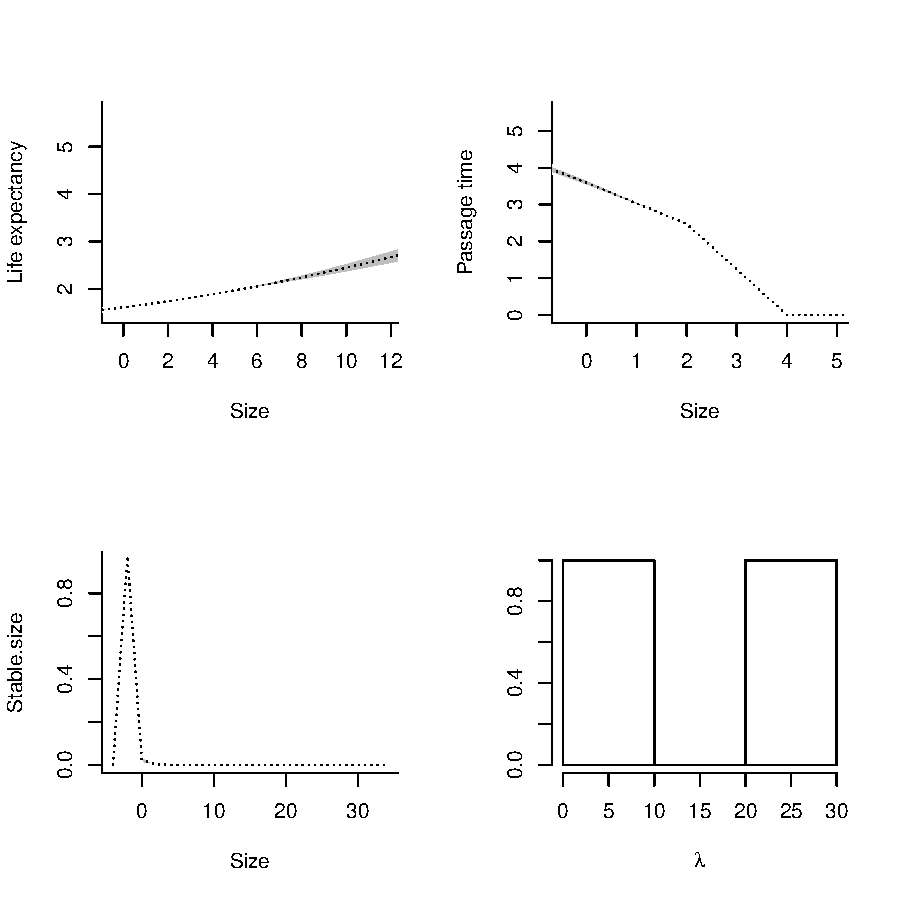
\includegraphics{IPMpack_Vignette-fig7}

\end{center}
\caption{Uncertainty in IPM output}
\label{fig:seven}
\end{figure}

This is a rather slow way of proceeding - a large number of IPMs are being stored in R's memory. A slightly more rapid approach is to use the function {\tt getIPMOutputDirect} that builds an IPM from a sample from the posterior, calculates relevant parameters, then over-writes this with a rebuilt IPM, etc.


\section{Building your own objects and methods}
If growth is best reflected by a saturating function, rather than the linear regression models provided, the user must define a new class of growth object:
\begin{Schunk}
\begin{Sinput}
> setClass("growthObjSaturate", representation(paras = "numeric", sd = "numeric"))
\end{Sinput}
\begin{Soutput}
[1] "growthObjSaturate"
\end{Soutput}
\end{Schunk}
Then define the functional form of the mean prediction, with relevant parameters: 
\begin{Schunk}
\begin{Sinput}
> fSaturate <- function(size, pars) { 
+     u <- exp(pmin(pars[1] + pars[2] * size, 50))
+     u <- pars[3] * 1/(1+u)
+     return(u)
+ }
\end{Sinput}
\end{Schunk}
where the third parameter indicates the asymptotic size. The user can then estimate the parameters by fitting this function to the data using a wrapper function and
{\tt optim}. 
\begin{Schunk}
\begin{Sinput}
> wrapSaturate <- function(par, dataf) { 
+     pred <- fSaturate(dataf$size, par[1:3])
+     ss <- sum((pred - dataf$sizeNext)^2, na.rm = TRUE)
+     return(ss)
+     }
> tmp <- optim(c(1, 1, 1), wrapSaturate, dataf = dff, method = "Nelder-Mead")
> tmp    
\end{Sinput}
\begin{Soutput}
$par
[1]  2.0279630 -0.3313762 10.3890754

$value
[1] 1111.277

$counts
function gradient 
     356       NA 

$convergence
[1] 0

$message
NULL
\end{Soutput}
\end{Schunk}

For simplicity, one can assume normally distributed errors: 

\begin{Schunk}
\begin{Sinput}
> resids <- fSaturate(dff$size, tmp$par) - dff$sizeNext
> sdSaturate <- sd(resids, na.rm = TRUE)
\end{Sinput}
\end{Schunk}

With these parameters, the user can then define the new growth object:

\begin{Schunk}
\begin{Sinput}
> gr1 <- new("growthObjSaturate")
> gr1@paras <- tmp$par
> gr1@sd <- sdSaturate
\end{Sinput}
\end{Schunk}

Finally, the user must define a method appropriate for this type of object. 

\begin{Schunk}
\begin{Sinput}
> setMethod("growth", c("numeric", "numeric", "numeric", "growthObjSaturate"), 
+           function(size, sizeNext, cov, growthObj){
+               mux <- fSaturate(size, growthObj@paras)
+               sigmax <- growthObj@sd
+               u <- dnorm(sizeNext, mux, sigmax, log = F)  
+               return(u);
+           })
\end{Sinput}
\begin{Soutput}
[1] "growth"
\end{Soutput}
\end{Schunk}
By putting {\tt growthObjSaturate} in the signature, R will use this particular method for all objects with this signature. Now, the user can go ahead and use all the other code as previously, without a need for further definitions. 

If the user wishes to fit a growth model with, for example, gamma errors, a similar approach can be used, but with `dgamma' instead of dnorm in the last line of growth method, and appropriate slots defined in the object, etc. 

\section*{Selected References}



\begin{itemize}
\item Caswell. 2001. Matrix population models: analysis, construction and interpretation. 2nd ed. Sinauer. Massachussetts, USA.

NA

\item Cochran \& Ellner. 1995. Simple methods for calculating age-based life history parameters for stage-structured populations. Ecological Monographs 62: 345-364.

\item Ellner \& Rees. 2006. Integral projection models for species with complex life-histories. American Naturalist 167: 410-428.

\item Metcalf, Horvitz, Tuljapurkar \& Clark. 2009. A time to grow and a time to die: a  new way to analyze the dynamics of size, light, age and death of tropical trees. Ecology 90: 2766-2778.

\item Rees \& Rose. 2002. Evolution of flowering strategies in Oenothera glazioviana: an integral projection model approach. Proc. Roy. Soc. Lond. Ser. B. 269: 1509-1515.

\item Ramula, Rees \& Buckley. 2009. Integral projection models perform better for small demographic data sets than matrix population models: a case study of two perennial herbs. Journal of Applied Ecology 46: 1048-1053.

\item Salguero-Gomez \& Plotkin. 2010. Matrix dimensionality bias demographic inferences: implications for comparative plant demography. The American Naturalist 176: 710-722

\item Tuljapurkar. 1990. Population Dynamics in Variable Environments. Springer. New York, USA.

\item Zuidema, Jongejans, Chien, During \& Schieving. 2010. Integral Projection Models for trees: a new parameterization and a validation of model output. Journal of Ecology 98: 345-355.


\end{itemize}

%\section{Extensions}

%\begin{itemize}
%\item  sensitivity / elasticity a la Carol Tulja
%\item stable size dist in stoch env
%\item survivorship in a stochastic environment
%\item density dependence generic functions
%\item age structure
%\item jim style multi-year census interval growth bayes
%\item loop analysis (see Zuidema in Ecology showing fast growing
%  trees contribute more)
%\end{itemize}


\end{document}

